\section{Рабочий проект}

\subsection{Модули, разработанные для реализации интерпретатора}

С целью обеспечить логическое разделение кода, во время его написания были разработаны модули, представляющие собой связанные друг с другом исходные файлы на языке C, составляющие функциональность интерпретатора.


\begin{figure}[h!t]
	\center{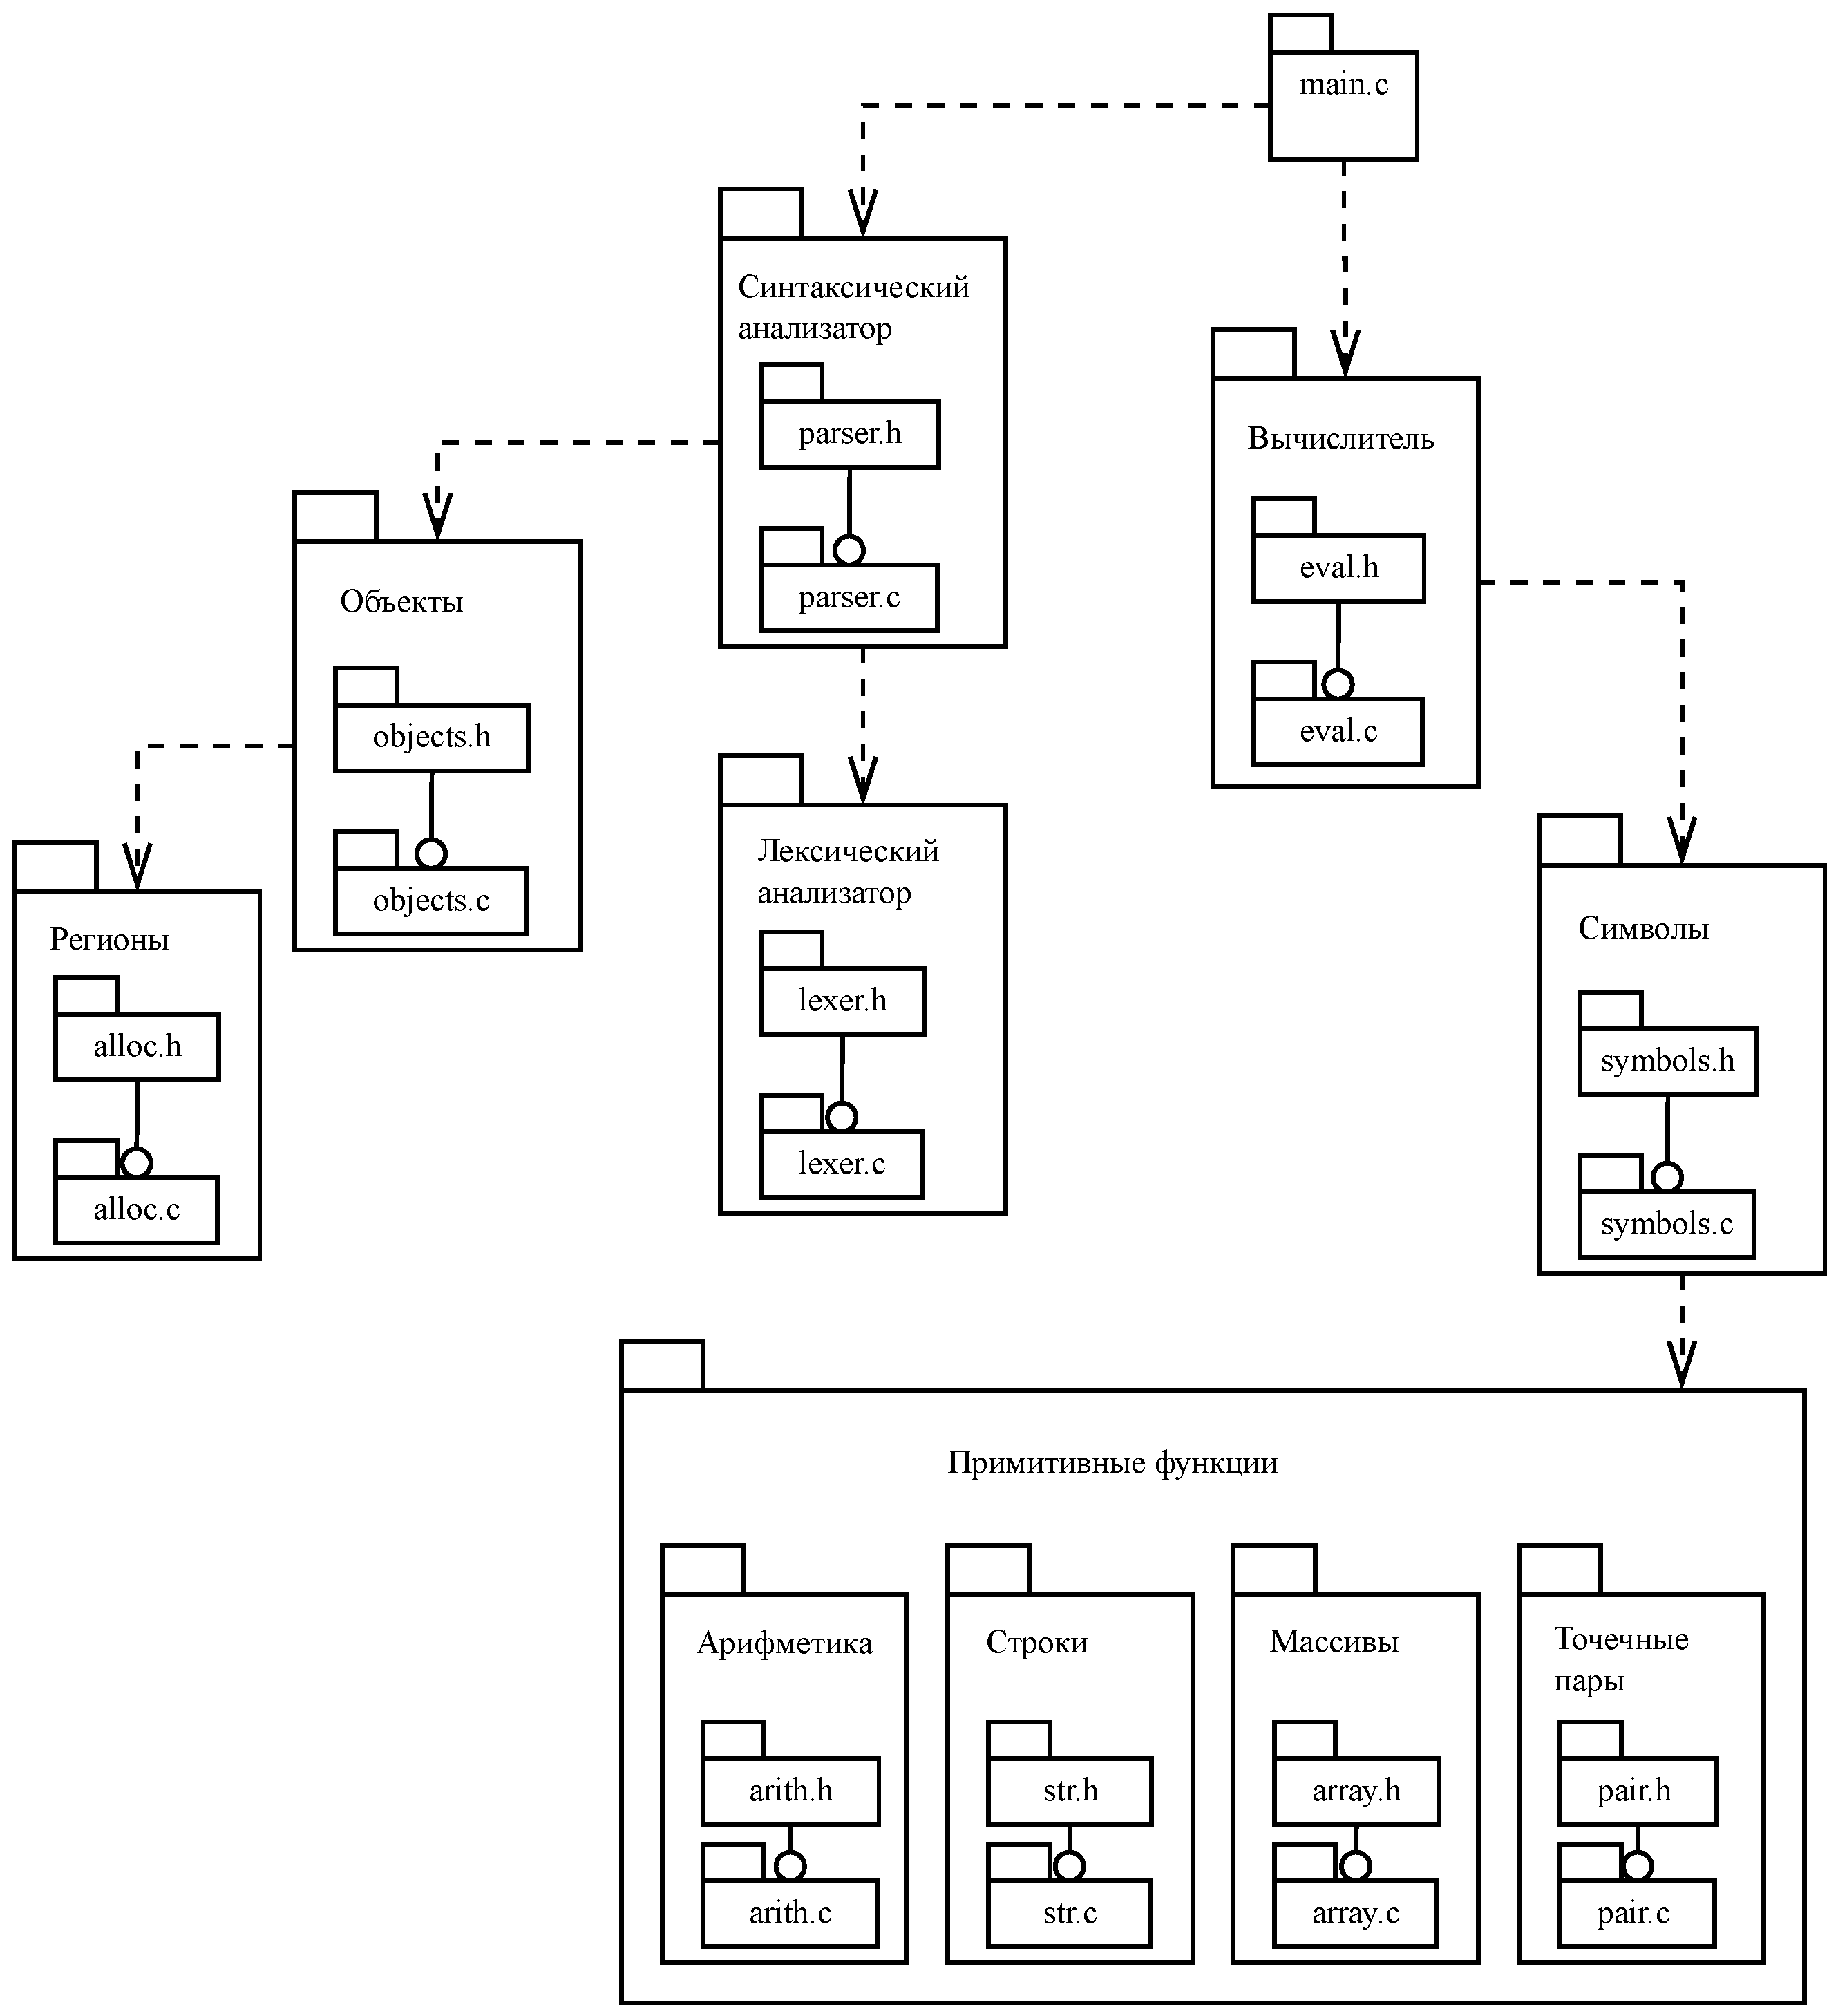
\includegraphics[width=1\linewidth]{uml_package}}
	\caption{Диаграмма пакетов интерпретатора}
	\label{uml_package:image}
\end{figure}

Эти файлы и их зависимость друг от друга продемонстрированы на рисунке \ref{uml_package:image} в виде UML-диаграммы пакетов \cite{e32}.

Перечень модулей представлен в таблице \ref{modules:table}, куда входят их имена, роль в структуре разрабатываемой ПС, а также описания выполняемых ими задач.

\begin{xltabular}{\textwidth}{|l|p{4cm}|X|}
	\caption{Модули интерпретатора\label{modules:table}} \\ \hline
	\centrow Имя & \centrow Роль & \centrow Задача \\ \hline
	\thead{1} & \thead{2} & \centrow 3 \\ \hline
	\endfirsthead
	\continuecaption{Продолжение таблицы \ref{modules:table}}
	\thead{1} & \thead{2} & \centrow 3 \\ \hline
	\finishhead
	main.c & Главный модуль & Выполняет инициализацию всех остальных модулей, организует работу между ЛА и исполнителем, запускает сборщик мусора, выполняет возвращение в точку до ошибки при её возникновении \\ \hline
	alloc.c & Модуль работы с регионами & Хранение массивов и строк реализовано через \quotes{регионы}, инструменты для управления которыми помещены в этот модуль \\ \hline
	objects.c & Модуль внутреннего объектного представления & Содержит функции, позволяющие создавать объекты и манипулировать ими \\ \hline
	arith.c & Модуль арифметических функций & Реализует примитивные арифметические функции \\ \hline
	str.c & Модуль работы со строками & Реализует инструменты для создания объектов-строк и манипуляции ими \\ \hline
	array.c & Модуль работы с массивами & Реализует инструменты для создания объектов-массивов и манипуляции ими \\ \hline
	symbols.c & Модуль работы с символами & Реализует инструменты для создания объектов-символов и манипуляции ими \\ \hline
	pair.c & Модуль работы с парами & Реализует инструменты для создания точечных пар и списков и манипуляции ими \\ \hline
	lexer.c & Лексический анализатор & Реализует все возможности, необходимые для анализа лексем и создания токенов на их основе \\ \hline
	parser.c & Синтаксический анализатор & Реализует все возможности, необходимые для формирования объектов внутреннего представления на основе токенов \\ \hline
	eval.c & Модуль исполнения & Исполняет s-выражения, связывая тем самым примитивные функции языка и объекты внутреннего представления \\ \hline
\end{xltabular}

\subsection{Спецификация модулей лексического и синтаксического анализаторов}

Для более глубокого раскрытия задач ЛА (lexer.c) и СА (parser.c) в таблицах \ref{modinfo_lexer_fields:table} - \ref{modinfo_parser_funcs:table} приведены поля и методы этих модулей с их именами, описаниями и типами входных и выходных данных.

\begin{xltabular}{\textwidth}{|l|p{3.5cm}|X|}
	\caption{Спецификация полей модуля \quotes{lexer.c}\label{modinfo_lexer_fields:table}}\\ \hline
	\centrow Имя & \centrow Тип & \centrow Описание \\ \hline
	\thead{1} & \thead{2} & \centrow 3 \\ \hline
	\endfirsthead
	\continuecaption{Продолжение таблицы \ref{modinfo_lexer_fields:table}}
	\thead{1} & \thead{2} & \centrow 3 \\ \hline
	\finishhead
	cur\_symbol & char & Символ, считанный последним (текущий символ) \\ \hline
	token & token\_t & Токен, генерируемый в момент лексического анализа (текущий токен) \\ \hline
	token\_error & int & Флаг, оповещающий парсер о возникновении ошибки при лексическом разборе. Если произошла ошибка, его значение -- 1, иначе 0 \\ \hline
	SYMBOL\_BUFFER\_SIZE & Целочисленная символическая константа & Задаёт размер буфера символов \\ \hline
	symbol\_buffer & char[] & Буфер символов, считанных из стандартного потока ввода. Имеет обратный порядок элементов. Размер буфера задаётся значением \quotes{SYMBOL\_BUFFER\_SIZE} \\ \hline
	buffer\_write\_pos & int & Текущая позиция записи в буфере символов \\ \hline
	buffer\_read\_pos & int & Текущая позиция чтения из буфера символов \\ \hline
\end{xltabular}

\begin{xltabular}{\textwidth}{|l|p{3.2cm}|X|}
	\caption{Спецификация методов модуля \quotes{lexer.c}\label{modinfo_lexer_funcs:table}}\\ \hline
	\centrow Имя & \centrow Ввод / вывод & \centrow Описание \\ \hline
	\thead{1} & \thead{2} & \centrow 3 \\ \hline
	\endfirsthead
	\continuecaption{Продолжение таблицы \ref{modinfo_lexer_funcs:table}}
	\thead{1} & \thead{2} & \centrow 3 \\ \hline
	\finishhead
	get\_cur\_char & > void & Считывает символ из потока ввода и помещает его в буфер. Когда буфер заполняется, производится сдвиг позиций чтения и записи \\ \hline
	unget\_cur\_char & > void & Возвращает позицию чтения назад на единицу и переприсваивает текущий символ \\ \hline
	is\_whitespace & < char c \linebreak > int & Проверяет является ли символ пробельным (пробел, перенос строки, табуляция) \\ \hline
	skip\_comment & > void & Пропускает все символы, пока не достигнет переноса строки или конца входного потока \\ \hline
	skip\_white\_space & > void & Выполняет пропуск при обнаружении пробельного символа или знака комментария, оперируя для этого функциями \quotes{is\_whitespace} \quotes{skip\_comment} \\ \hline
	is\_digit & < char c \linebreak > int & Проверяет является ли символ \quotes{c} цифрой (от 0 до 9). Если да -- возвращает 1, иначе 0 \\ \hline
	is\_alpha & < char c \linebreak > int & Проверяет является ли символ \quotes{c} буквой латинского алфавита в верхнем или нижнем регистре. Если да -- возвращает 1, иначе 0 \\ \hline
	is\_symbol & < char c \linebreak > int & Проверяет является ли символ \quotes{c} разрешённым (+-*/=\_\&|<>). Если да -- возвращает 1, иначе 0 \\ \hline
	is\_hex\_symbol & < char c \linebreak > int & Проверяет является ли символ \quotes{c} одним из шестнадцатеричных символов от \quotes{a} до \quotes{f} и от \quotes{A} до \quotes{F} \\ \hline
	is\_delimeter & < char c \linebreak > int & Проверяет является ли символ \quotes{c} разделителем: открывающая и закрывающая скобки, обратная косая черта, двойная кавычка, пробельный символ, конец потока \\ \hline
	hex\_num & > int & Преобразует шестнадцатеричное число из потока ввода в десятичное и возвращает его \\ \hline
	get\_float\_num & > void & Принимает целую часть \quotes{int\_num} от вещественного числа и считывает оставшиеся после точки числа. Преобразует имеющиеся данные в число с плавающей точкой в формате целочисленного (int) и возвращает его \\ \hline
	get\_num & > int & Считывает из потока ввода число в десятичной или шестнадцатеричной системе счисления и приводит его к десятичной. Записывает его в переменную \quotes{cur\_num}, после чего возвращает \\ \hline
	get\_symbol & < char *cur\_str \linebreak > void & Считывает имя символа из \quotes{cur\_str} и проверяет его на корректность. Если не корректное -- задаёт для \quotes{token\_error} значение 1 и выводит ошибку \\ \hline
	get\_string & < char *cur\_str \linebreak > void & Считывает строку, обрамлённую двойными кавычками, из \quotes{cur\_str}. Если отсутствует закрывающая кавычка, выводит ошибку и устанавливает значение \quotes{token\_error} в 1\\ \hline
	get\_comma & > token\_t & Обрабатывает лексему \quotes{,} или \quotes{,@} из входного потока, формирует для неё токен и возвращает его \\ \hline
	get\_sharp & > token\_t & Обрабатывает лексему \quotes{\#} или \quotes{\# \textbackslash} из входного потока, формирует для неё токен и возвращает его \\ \hline
	get\_token & > token\_t* & Считывает лексему из потока ввода, формирует на её основе токен и возвращает его, используя для этого все вышеперечисленные функции
	
\end{xltabular}

\begin{xltabular}{\textwidth}{|l|p{3.5cm}|X|}
	\caption{Спецификация полей модуля \quotes{parser.c}\label{modinfo_parser_fields:table}}\\ \hline
	\centrow Имя & \centrow Тип & \centrow Описание \\ \hline
	%\thead{1} & \thead{2} & \centrow 3 \\ \hline
	%\endfirsthead
	%\continuecaption{Продолжение таблицы \ref{modinfo_parser_fields:table}}
	%\thead{1} & \thead{2} & \centrow 3 \\ \hline
	\finishhead
	token\_error & extern int & Флаг, устанавливаемый лексером для оповещения парсера о возникновении ошибки при лексическом разборе. Если произошла ошибка, его значение -- 1, иначе 0 \\ \hline
	cur\_token & token\_t & Последний полученный токен (текущий токен)
\end{xltabular}

\begin{xltabular}{\textwidth}{|l|p{3.2cm}|X|}
	\caption{Спецификация методов модуля \quotes{parser.c}\label{modinfo_parser_funcs:table}}\\ \hline
	\centrow Имя & \centrow Ввод / вывод & \centrow Описание \\ \hline
	\thead{1} & \thead{2} & \centrow 3 \\ \hline
	\endfirsthead
	\continuecaption{Продолжение таблицы \ref{modinfo_parser_funcs:table}}
	\thead{1} & \thead{2} & \centrow 3 \\ \hline
	\finishhead
	strupr & < char *str \linebreak > char* & Преобразует строку \quotes{str} в верхний регистр и возвращает её \\ \hline
	parse\_quote & < char *quote\_sym \linebreak > object\_t & Считывает s-выражение из потока ввода и помещает его как аргумент в вызов функции цитирования или квазицитирования, после чего возвращает полученный объект-список \\ \hline
	parse\_element & < type\_t type, void *data, tokentype\_t t\_type \linebreak > object\_t & Обрабатывает элемент списка, формирует на его основе объект и возвращает \\ \hline
	parse\_list & > object\_t & Обрабатывает список, формируя объекты на основе входящих в него токенов, пока не будет достигнута закрывающая скобка. По окончании возвращает указатель на сформированный объект-список \\ \hline
	parse\_array & > object\_t & Формирует объект-массив на основе входящих в него токенов  \\ \hline
	parse & > object\_t & Считывает токены, составляющие s-выражение, формирует на их основе объект-список и возвращает его  \\ \hline
\end{xltabular}


\subsection{Модульное тестирование разработанного интерпретатора}

Для тестирования разработанной программной системы были созданы пакеты модульных и системного тестов.

Модульные тесты вызывают функции компонентов интерпретатора с некоторыми параметрами и проверяют полученные на их выходе результаты с ожидаемыми. Этот тип тестов позволяет достаточно детально проверить работу не только какого-либо механизма ПС, но и функций, которые этот механизм формируют \cite{e14}.

На каждый модуль системы был разработан собственный пакет тестов, где почти каждая функция проверяется несколькими способами, покрывая проверками все их сценарии работы.

Один из них, тест модуля символов (test\_symbols.c), продемонстрирован в виде таблицы \ref{modulet:table}, содержащей наименование тестируемой функции модуля, тестовый случай и ожидаемый результат, а также краткое описание принципа работы теста.

\begin{xltabular}{\textwidth}{|p{4cm}|p{4cm}|X|}
	\caption{Тестовые случаи для модуля \quotes{symbols.c}\label{modulet:table}}\\ \hline
	\centrow Имя & \centrow Ввод/вывод & \centrow Цель проверки \\ \hline
	\thead{1} & \thead{2} & \centrow 3 \\ \hline
	\endfirsthead
	\continuecaption{Продолжение таблицы \ref{modulet:table}}
	\thead{1} & \thead{2} & \centrow 3 \\ \hline
	\finishhead
	Сравнение двух строк (compare\_str) & < \quotes{abc}, \quotes{abc} \linebreak > 1 \linebreak < \quotes{abc}, \quotes{abc1} \linebreak > 0 & Тестовый случай охватывает варианты с совпадающими и несовпадающими строками, когда на выходе единица и ноль соответственно \\ \hline
	Создание символа (find\_symbol) & < \quotes{ab} \linebreak > Объект-символ с именем \quotes{ab} \linebreak < \quotes{a} \linebreak > Объект-символ с именем \quotes{a} & Символ с заданным именем отсутствует в таблице символов, потому будет создан. Тестовый случай проверяет, что имя созданного символа соответсвует заданному \\ \hline
	Тест на поиск символа по пустой строке (поочерёдно для find\_symbol и check\_symbol) & < \quotes{} \linebreak > NULL & Тестовый случай проверяет, что при получении пустой строки, она будет обработана особым образом и будет возвращено значение NULL \\ \hline
	Строка для поиска символа имеет недопустимую длину (поочерёдно для find\_symbol и check\_symbol) & < Строка длиной 82 символа \linebreak > NULL & Тестовый случай проверяет, что при получении функцией строки, длиной превосходящей допустимую -- более 81 символа, она будет обработана особенным образом и из неё вернётся значение NULL \\ \hline
	Создание символа по строке максимальной длины (find\_symbol) & < Строка длиной 81 символ \linebreak > Новый символ с заданным именем & Тестовый случай проверяет, что при обработке функцией строки максимальной длины не происходит ошибка неучтённой единицы \\ \hline
	
	Поиск символ по строке максимальной длины (check\_symbol) & < Строка длиной 81 символ \linebreak > Найденный по заданному имени символ & Тестовый случай проверяет, что при обработке функцией строки максимальной длины не происходит ошибка неучтённой единицы \\ \hline
	Регистрация функции (register\_func) & < "TEST", test \linebreak > & Регистрация функции прошла успешно и можно получить её по имени "TEST" и указатель на её тело соответствует переданному -- test. \\ \hline
	Создание и получение символа (check\_symbol и find\_symbol) & < "f" \linebreak > NULL \linebreak > Новый символ с именем "f" \linebreak > Созданный ранее символ с именем "f" & Проверив с помощью check\_symbol отсутствие символа, он будет создан с применением find\_symbol и проверка проведётся повторно. Тем самым производится контроль за корректностью работы двух функций вместе \\ \hline
	Разные символы с одинаковым хеш-значением (hash и find\_symbol)& < \quotes{PJ}  \quotes{452}  "\textbackslash xe4\textbackslash x44\textbackslash x8a" \linebreak > Символы не равны & Хеш-значения, вычисленные на основе строк из параметров, одинаковы, но объекты-символы, сформированные по ним, указывают на разные области памяти
\end{xltabular}

Вывод в консоль результатов выполнения этих тестов также показан на рисунке \ref{modul_test_res:image}.
\begin{figure}[H]
	\center{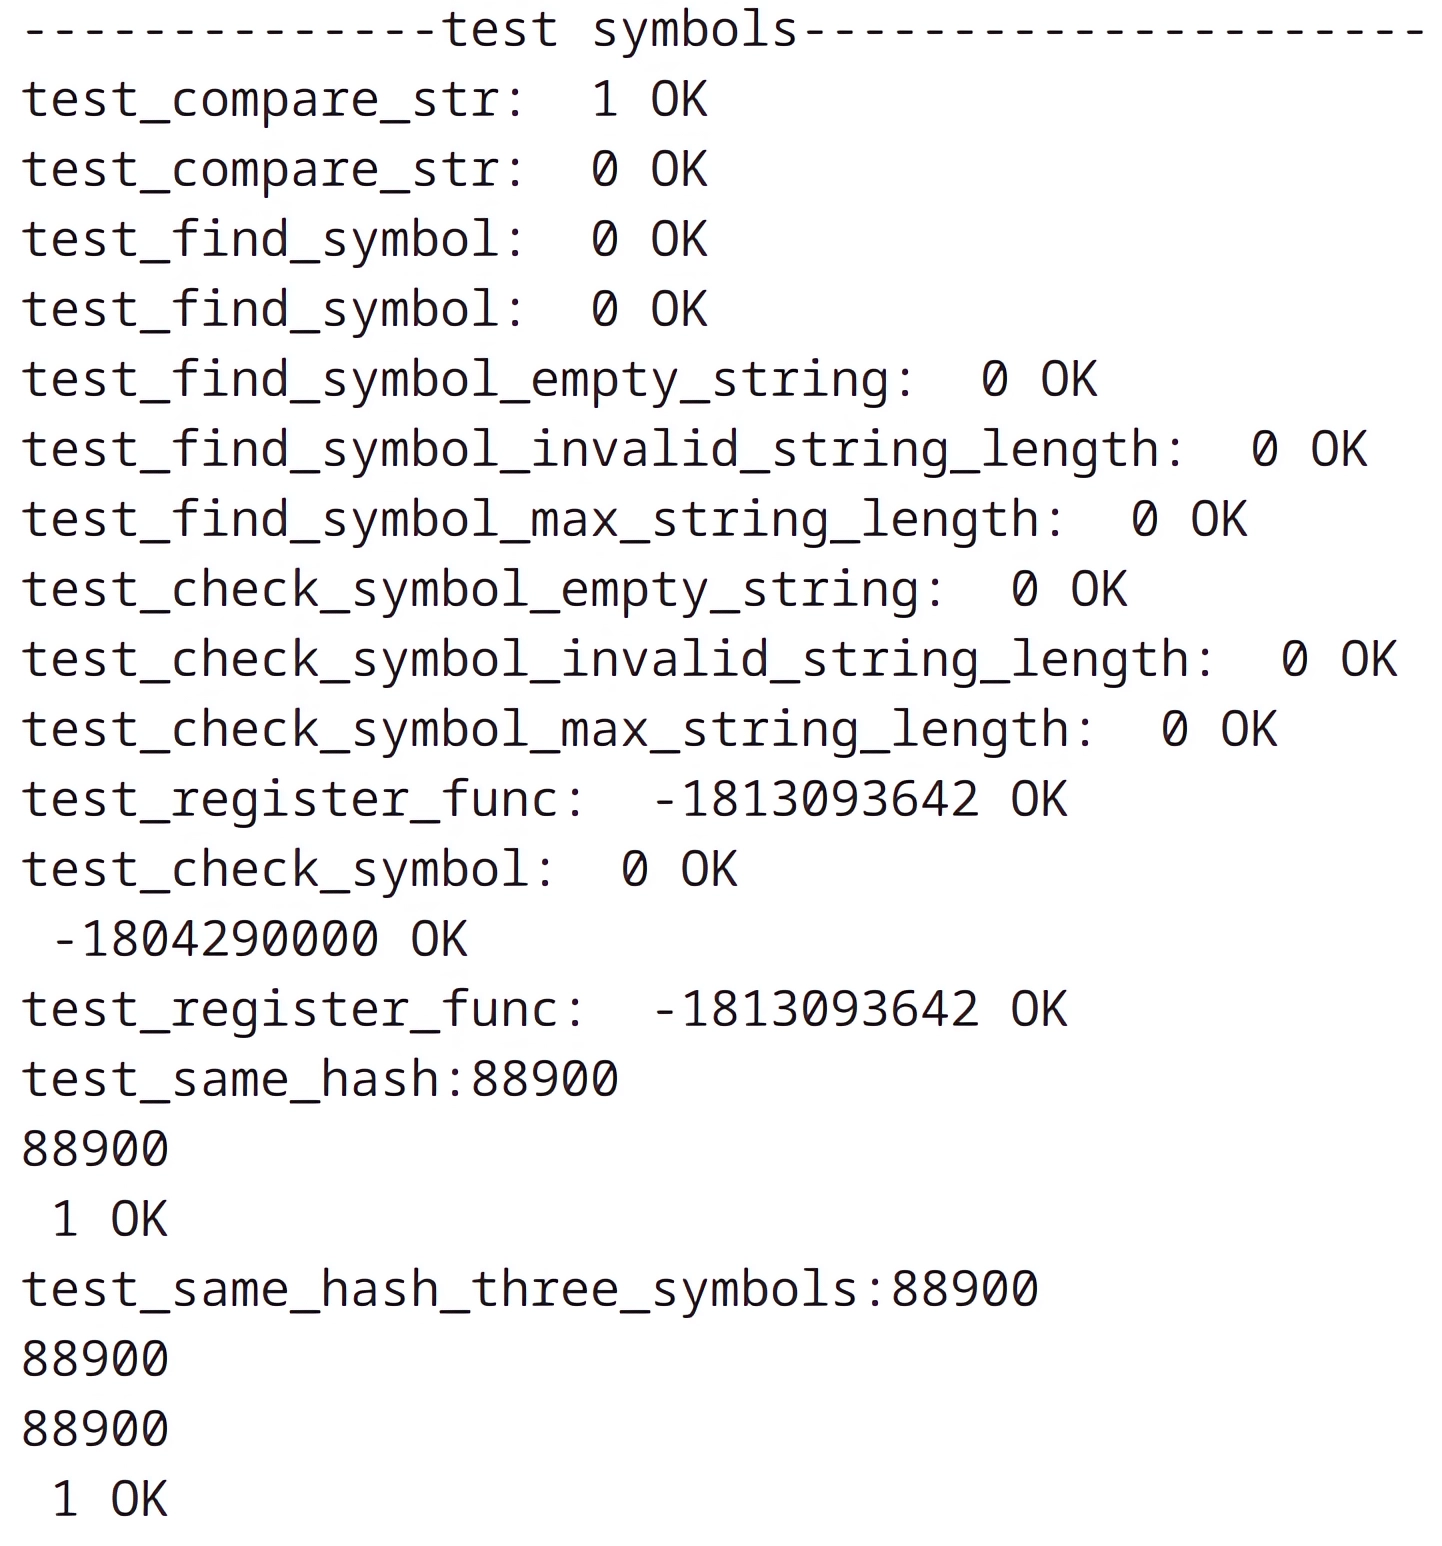
\includegraphics[width=1\linewidth]{modul_test_res}}
	\caption{Вывод в консоль результатов выполнения модульного теста test\_symbols.c}
	\label{modul_test_res:image}
\end{figure}

\subsection{Системное тестирование разработанного интерпретатора}

Системные же тесты проверяют работу ПС по принципу чёрного ящика, с теми же возможностями, что есть у пользователя. Этот метод подходит для проверки корректности работы интерпретатора в целом \cite{e15}. Суть подхода заключается в запуске передаваемого в виде строки программного кода и сравнения выведенных в консоль результатов его выполнения с эталонными.

Для тестирования используется bash-скрипт \quotes{sys\_test}. При его вызове программный код подаётся в двойных кавычках первым аргументом, а эталонный (ожидаемый) результат аналогичным образом вторым аргументом. При совпадении фактического и ожидаемого результата, в поток вывода \cite{e28} попадёт \quotes{OK}, иначе \quotes{FAIL}. Запуск тестового пакета необходимо производить в консольном интерфейсе, запись результатов при этом будет происходить в стандартный поток вывода консоли.

Несколько тестов из пакета системного тестирования представлены на рисунке \ref{system_test_code:image}.

\begin{figure}[ht]
	\center{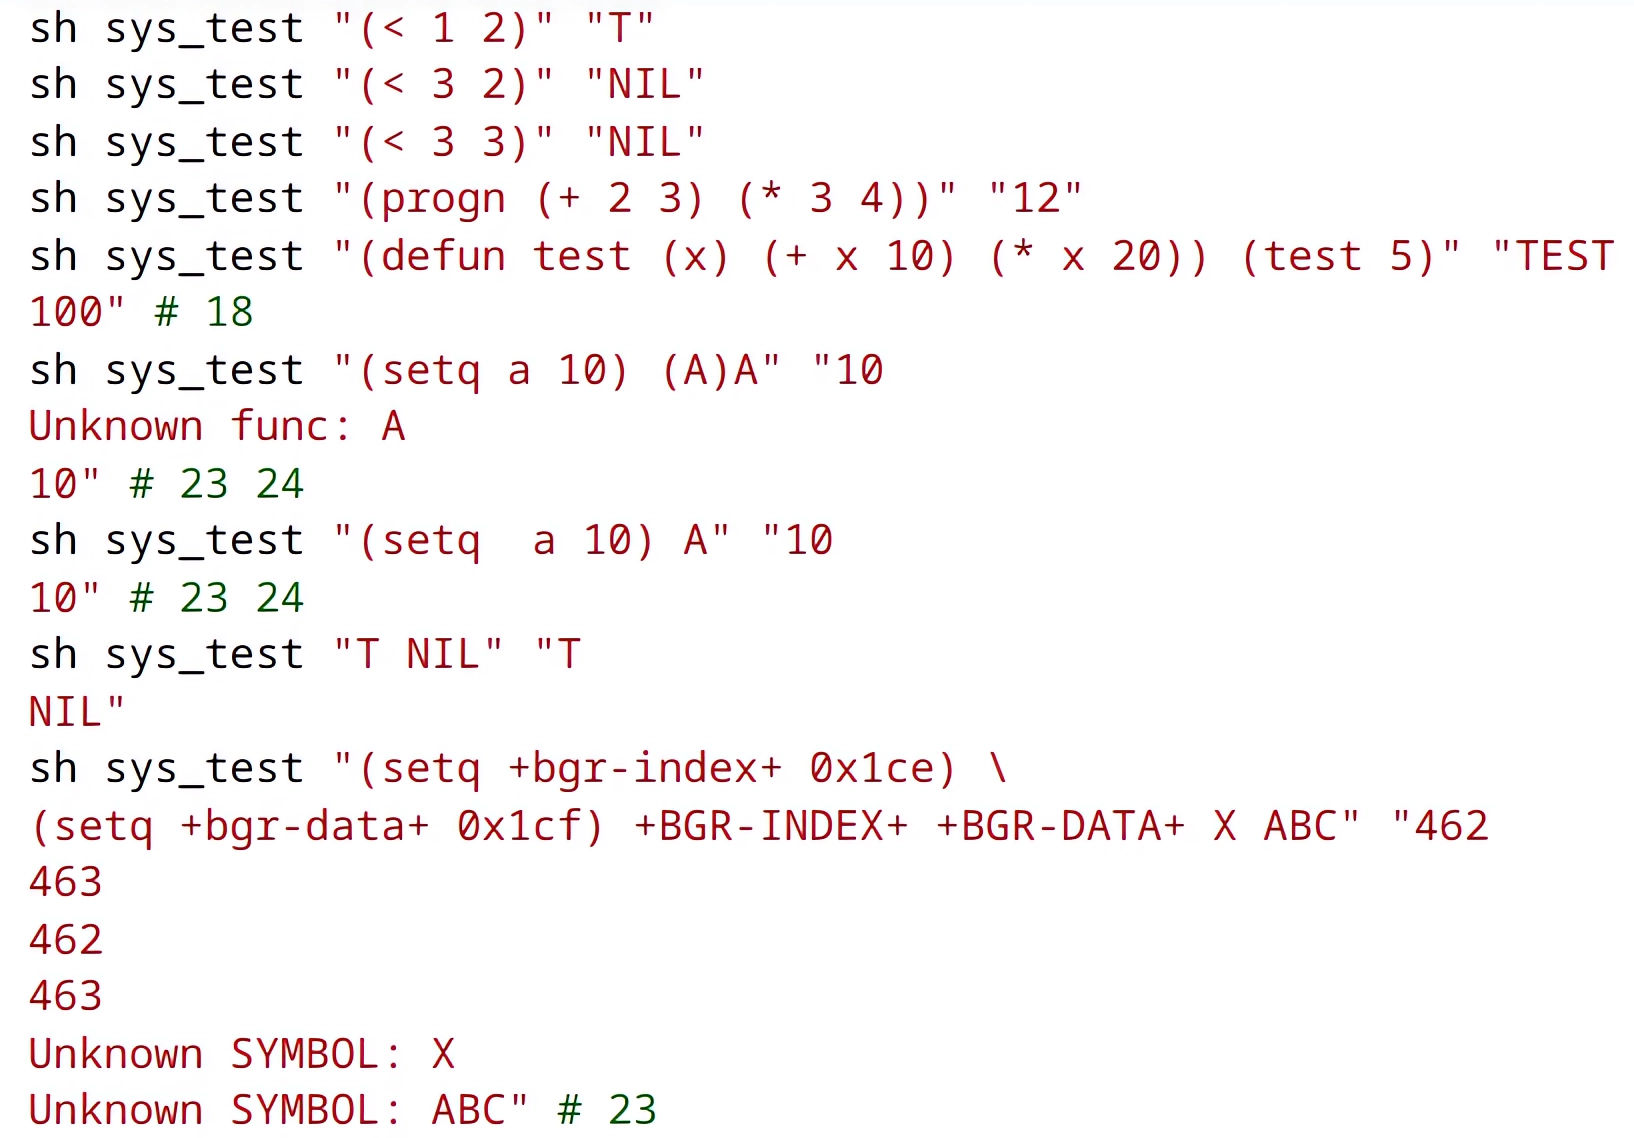
\includegraphics[width=1\linewidth]{system_test_code}}
	\caption{Часть тестов из пакета системного тестирования}
	\label{system_test_code:image}
\end{figure}

Вывод в консоль результатов выполнения этих тестов так же показан на рисунке \ref{system_test_res:image}.

\begin{figure}[H]
	\center{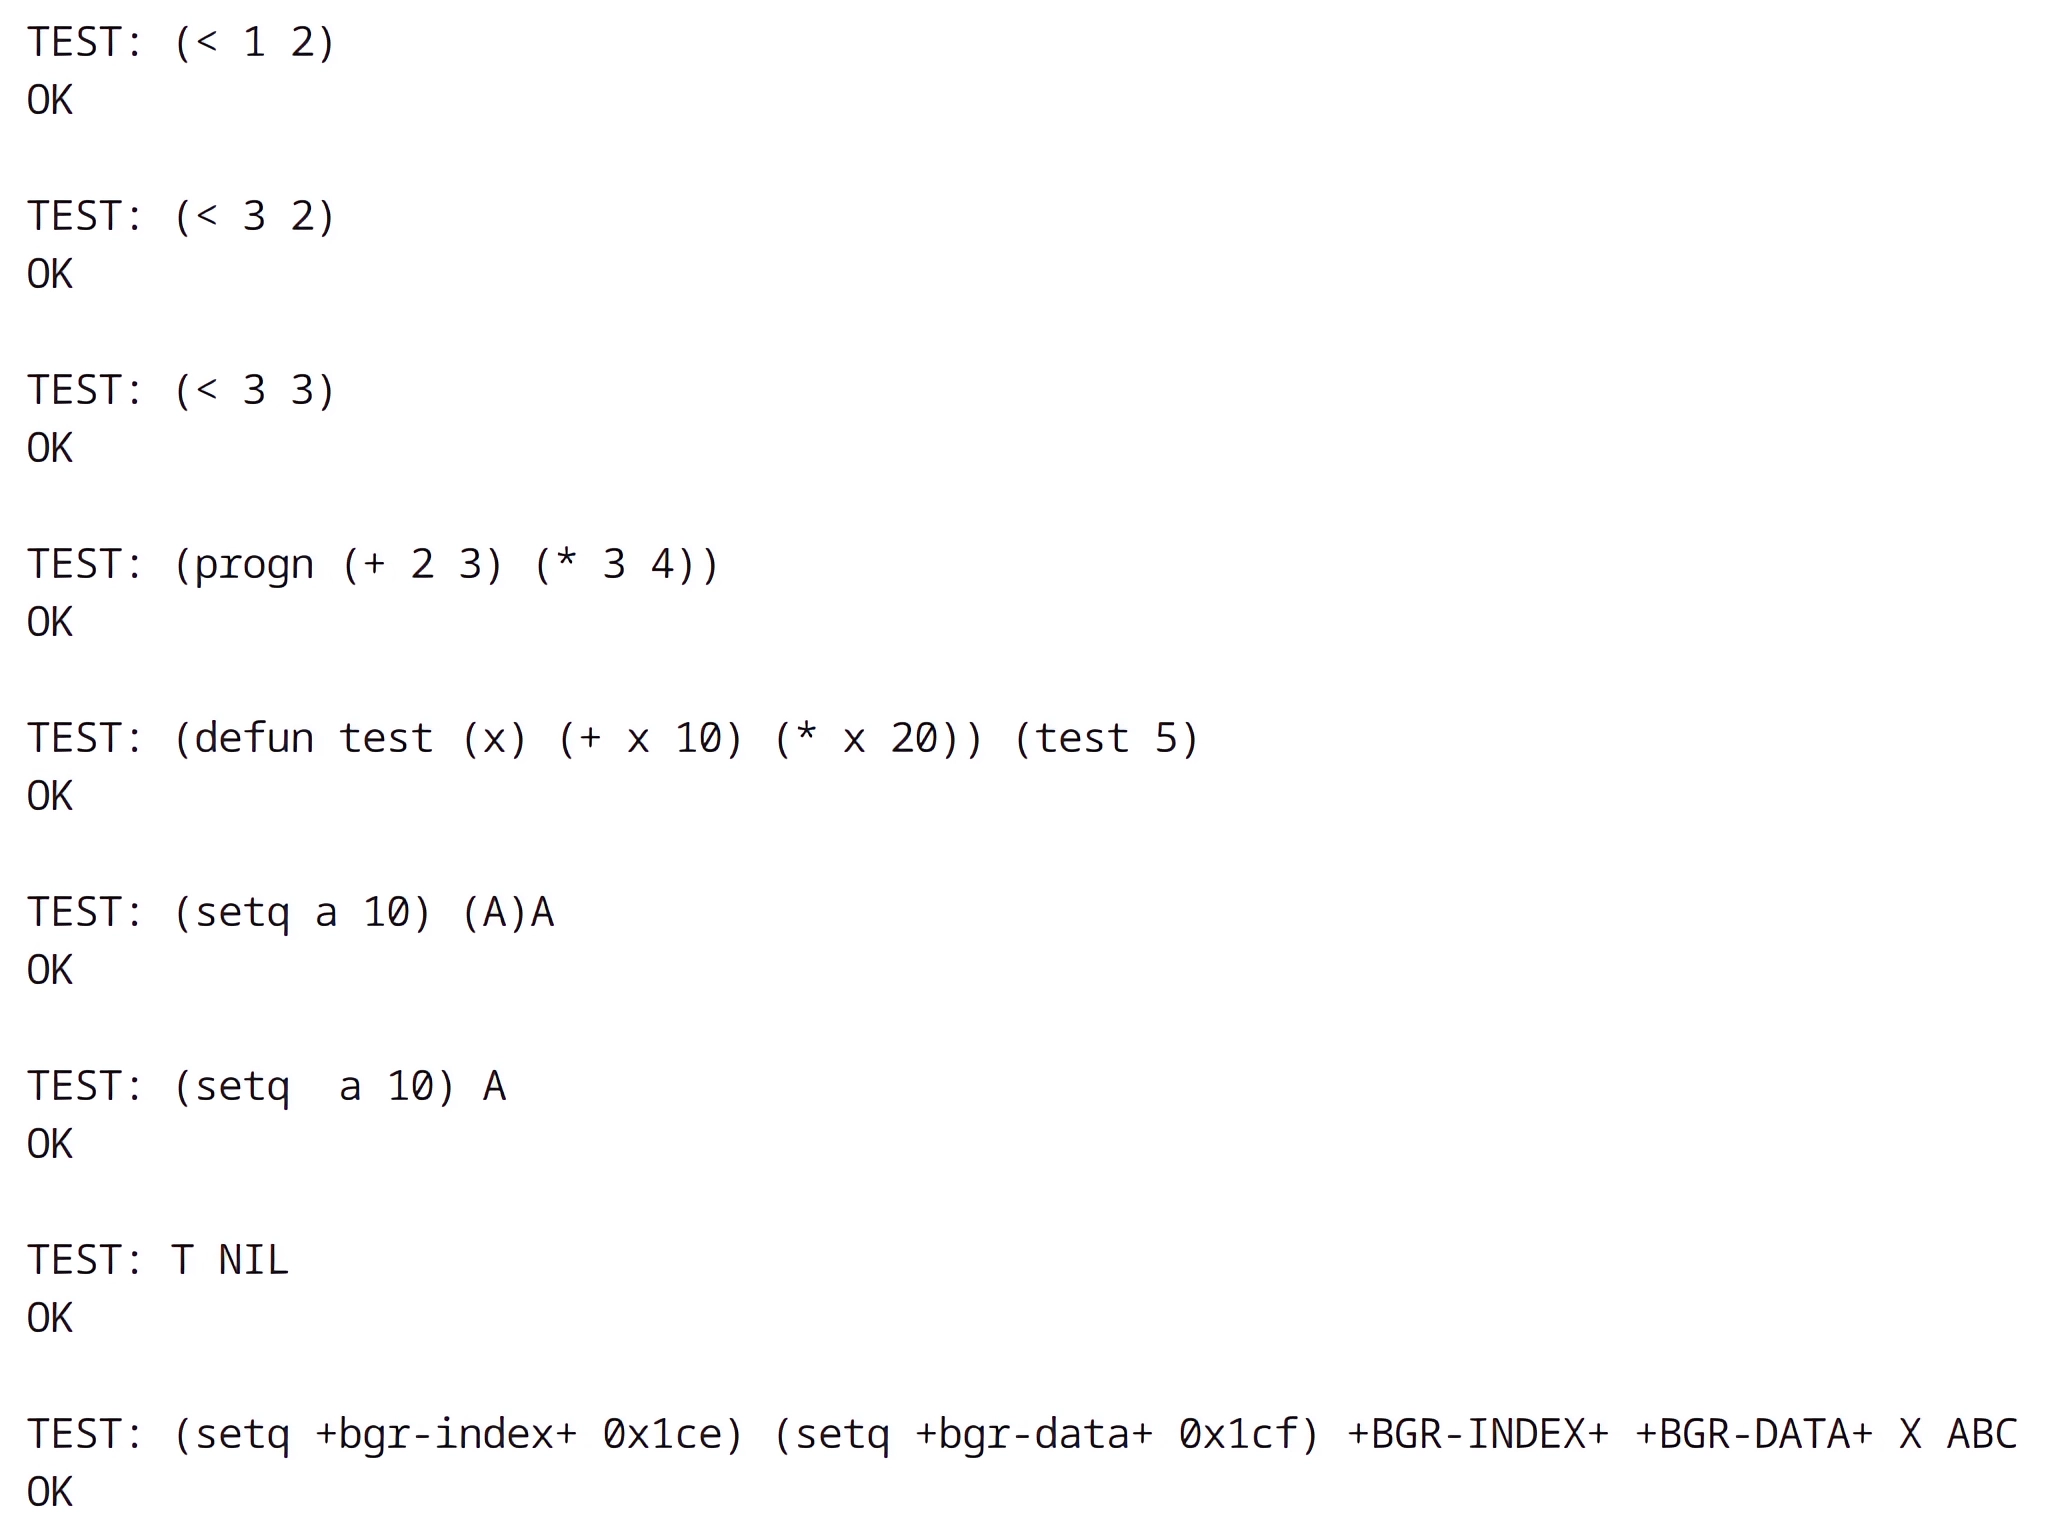
\includegraphics[width=1\linewidth]{system_test_res}}
	\caption{Вывод в консоль результатов выполнения системных тестов}
	\label{system_test_res:image}
\end{figure}

Алгоритм работы тестового пакета:

\begin{enumerate}
\item Определяем переменные \quotes{IN}, \quotes{OUT}, и \quotes{OUT\_EXP}, используемые для хранения путей к временным файлам для хранения кода, фактических результатов и ожидаемых результатов соответственно. В дальнейшем "IN" будет использоваться для передачи программного кода на выполнение, а \quotes{OUT}" и \quotes{OUT\_EXP} для сравнения результатов;

\item Выводим строку \quotes{TEST: \$1}, где \quotes{\$1} — выполняемый программный код;

\item Записываем строку выполняемого программного кода в файл, путь к которому задан в переменной \quotes{IN}. Аналогично поступаем с ожидаемым результатом, но берём путь из переменной \quotes{OUT\_EXP};

\item Запускаем интерпретатор, перенаправляя в его поток вввода данные из файла \quotes{IN}, а также перенаправляем поток вывода в \quotes{OUT};

\item Сравниваем данные из файлов \quotes{OUT} и \quotes{OUT\_EXP}, используя встроенную в систему утилиту \quotes{diff} \cite{e24}. Если файлы идентичны, выводим \quotes{OK} -- успешное завершение теста, иначе \quotes{FAIL} -- несоответствие ожидаемого вывода фактическому.

\item Выводим пустую строку, создав тем самым перенос строки для визуального разделения результатов тестов.

\end{enumerate}

\subsection{Пример использования метапрограммирования для сокращения размера исходного кода}

Приведу пример программы, написанной на ДЯП, позволяющей сокращать размер исходного кода за счёт использования макросов.

Напишу макрос для ветвления, позволяющий выполнять первый исход, если результат условия ложный, иначе второй исход. Для этого реализуем три макроса:

Напишу макросы для следующих функций:
\begin{itemize}
	\item if: для выполнения первого исхода при истинном условии и второго иначе, разработаю на основе встроенного в язык оператора ветвления \quotes{cond};
	\item not: для инверсии булевых значений \quotes{T} и \quotes{NIL};
	\item nif: объединяющий \quotes{if} и \quotes{not} для достижения поставленной цели.
\end{itemize}

Реализация макросов:
\begin{lstlisting}[language=Lisp, frame=none]
	(defmacro if (test true false)
	`(cond (,test ,true)
	(t ,false)))
	
	(defmacro not (test)
	`(if ,test nil t))
	
	(defmacro nif (test true false)
	`(if (not ,test) ,true ,false))
\end{lstlisting}

Пример использования:
\begin{lstlisting}[language=Lisp, frame=none]
	(setq a 0)
	
	(nif (> 5 3)
	(setq a (+ a 1))
	(setq a (+ a 2)))
\end{lstlisting}

Если бы тот же самый пример был написан с применением \quotes{cond}:
\begin{lstlisting}[language=Lisp, frame=none]
	(setq a 0)
	
	(cond ((if (> 5 3) nil t)
	(setq a (+ a 1)))
	(t (setq a (+ a 2))))
\end{lstlisting}

Код, написанный с использованием nif, проще структурно, потому легче для понимания, и его кодовая запись короче.

Таким образом, с использованием разработанного макроса \quotes{nif} были достигнуты сокращение кода и его упрощение для чтения.

\subsection{Сборка программной системы}
Для компиляции созданной ПС были разработаны два файла сборки \quotes{makefile} \cite{e8}, реализующие разные варианты сборки интерпретатора.

Первый, расположенный в корневой папке разработанного интерпретатора, компилирует все модули интерпретатора в один готовый к использованию исполняемый файл. Для запуска сборки используется команда \quotes{make build}. В результате в той же папке будет сформирован файл \quotes{cl-inter}. Теперь можно запустить интерпретатор с нужным файлом исходного кода программы, передав путь до него в качестве параметра. Например: \quotes{cl-inter ./script}.

Второй, \quotes{test}, предназначен для запуска модульных и системных тестов, при этом, в случае модульного тестирования, в скомпилированный файл входят только необходимые для тестируемого модуля компоненты. Расположен в папке test, где также находятся все файлы тестов. При вызове \quotes{make test} поочерёдно будут собираться и выполняться все разработанные модульные и системный тесты. Исполняемые файлы при этом будут помещены в директорию ОС для временных файлов - \quotes{/tmp} \cite{e25}.